\chapter{Testes e Resultados}\label{cap:conclusão}

Neste capítulo será abordado os testes e resultados dos sensores, consumo de bateria e tempo de resposta do sistema embarcado e aplicativo \textit{Android}.

\section{Aplicação}

Nesta seção será discutida os valores encontrados na realização dos testes no aplicativo além de seu consumo e tempo de resposta para a notificação.

\subsection{\textbf{Sensores}}


Antes do desenvolvimento do protótipo do projeto foi desenvolvido um aplicativo para monitoramento exclusivamente dos sensores acelerômetro e giroscópio no \textit{Android}. O intuito deste aplicativo era observar o desempenho e o tempo de resposta dos sensores utilizados. Os testes foram realizados em um celular \textit{Android} 8.1 de modelo \textit{Zenfone} 4 ZE554KL,  o celular foi submetido a um teste de  8 horas para verificar o consumo da bateria e mais  um teste de 3 horas para a mensuração o comportamento dos sensores no trajeto até a faculdade.


No primeiro cenário o celular ficou com o aplicativo executando durante um período de 8 horas, nessas 8 horas  foram realizados movimentos com o aparelho e  períodos inertes. Este teste foi executado durante 3 dias para verificar seu comportamento.

No segundo cenário o aplicativo foi acionado durante o trajeto diário sendo assim o aplicativo  ficou exposto aos movimento do veículo, ao final do trajeto o aplicativo armazena todos os dados coletados e é encerrado. Este teste foi repetido durante uma semana.


Com o teste de uso do aplicativo em \textit{background} durante o período de 8 horas foi possível observar o consumo do celular chegando ao valor médio de 8 mAh  este dado de consumo foi retirado do próprio aparelho pois o sistema  o Android disponibiliza um relatório de consumo de energia de cada aplicação sendo executada no sistema. Com isto é possivel perceber um consumo muito baixo para um celular com autonomia de  3300 mAh, representando um consumo de 0,24\% da aplicação. 



No segundo teste foram coletados mais de dez mil amostras tanto para o acelerômetro quanto para o giroscópio, todos com o tempo mínimo de leitura de  100ms e sendo executados paralelamente. No entanto este tempo mínimo não se provou verdadeiro com os dados adquiridos. Realizando uma média dos valores coletados foi possivel perceber que o giroscopio possui mais que 400\% do valor minimo e o acelerometro mais que 20\%. A Tabela 2 mostra a média de todas as amostras, alem disto a Tabela 3 mostra uma amostra dos dados coletados.  




\begin{table}[]
    \centering
    \caption{Tabela com valores médios do giroscopio e acelerometro}
    \begin{tabular*}{\textwidth}{l@{\extracolsep{\fill}}cccc}
\toprule
{} &           tempo(ms) &  amostras  & tipo\\
\midrule
0 &  475.57 &  98638035 &  giroscpio \\
0 &  122.89 &  118510710 &  acelerometro \\
\bottomrule
\end{tabular*}

\end{table}



\begin{table}[]
    \centering
    \caption{Amostra dos dados coletados}

\begin{tabular*}{\textwidth}{l@{\extracolsep{\fill}}lrrrrrl}
\toprule
{} &     pk &         x &         y &         z &  tempo(ms) &          tipo \\
\midrule
0 &  11554 &  0.239120 & -0.123550 & -0.058319 &        396 &    giroscopio \\
1 &  11555 & -0.127335 & -0.287064 & -0.117981 &        322 &    giroscopio \\
2 &  11556 & -0.193375 &  0.315353 &  0.053528 &        383 &    giroscopio \\
3 &  11557 &  0.234863 & -0.219421 &  0.080704 &        517 &    giroscopio \\
4 &  11558 &  0.017014 &  0.067139 &  0.057800 &        349 &    giroscopio \\
0 &  26036 & -0.780502 &  6.909668 &  7.022186 &        100 &  acelerometro \\
1 &  26037 & -0.790085 &  7.223312 &  6.564896 &        146 &  acelerometro \\
2 &  26038 & -0.462067 &  7.565689 &  6.313507 &        192 &  acelerometro \\
3 &  26039 & -0.258560 &  7.821869 &  6.016632 &        137 &  acelerometro \\
4 &  26040 & -0.100555 &  7.596802 &  2.372650 &        136 &  acelerometro \\
\bottomrule
\end{tabular*} 
\end{table}




Com os dados adquiridos foi  possível notar que, o celular consegue coletar 10 amostras dos sensores a cada segundo em média sendo que, a cada quatro amostras coletadas pelo acelerômetro é feita a coleta de uma amostra do giroscópio. Sendo assim, é possível concluir que o giroscópio possui um tempo médio de 500ms e cerca de 125ms para cada leitura do acelerômetro. Com este estudo foi possível gerar, ao todo, 108 mil amostras coletadas em 3 horas de testes.

Com isto foram gerados os gráficos para monitorar a resposta dos sensores em cada eixo. A Figura 33 demonstra os eixos em relação a um celular .

 \begin{figure}[H]

\begin{center}
     \caption{Eixos Android}
  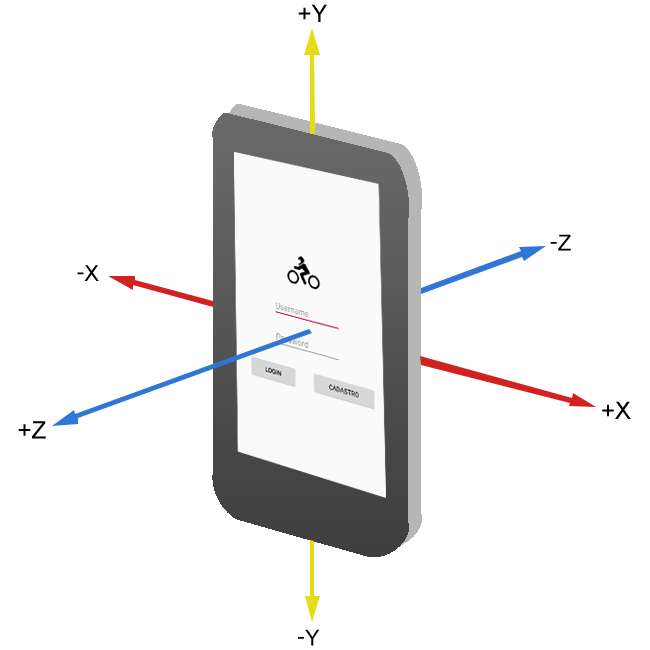
\includegraphics[width=70mm]{images/Cap5/eixos_anjo.png}
\end{center}
 \scriptsize Fonte: Os autores
  
\end{figure}


Com os dados adquiridos foi possível gerar gráficos individuais,  podendo visualizar o comportamento de cada eixo individualmente. A Figura 34 demonstra o gráfico em relação ao eixo X,Y,Z do acelerômetro.


 \begin{figure}[H]

\begin{center}
     \caption{Gráfico eixos do acelerometro}
  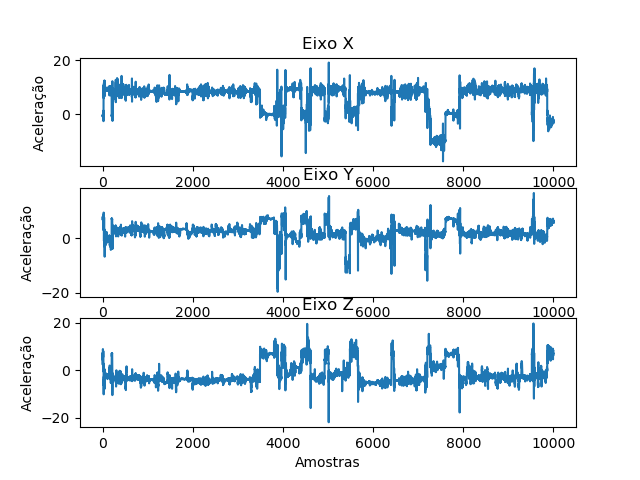
\includegraphics[width=150mm]{images/Cap5/acelerao_3_eixos.png}
\end{center}
 \scriptsize Fonte: Os autores
  
\end{figure}



O eixo Y é correspondente à aceleração, e o eixo X responsável pelo número de amostras coletadas. Com a Figura 35 é possível perceber que o celular   possui uma força média de 1G mesmo estando em movimento durante  todo o percurso, os pontos de variações são ações de pegar o celular na mão e realização de gesto ao utilizá-lo.


 \begin{figure}[H]

\begin{center}
     \caption{Gráfico da aceleração dos sensores}
  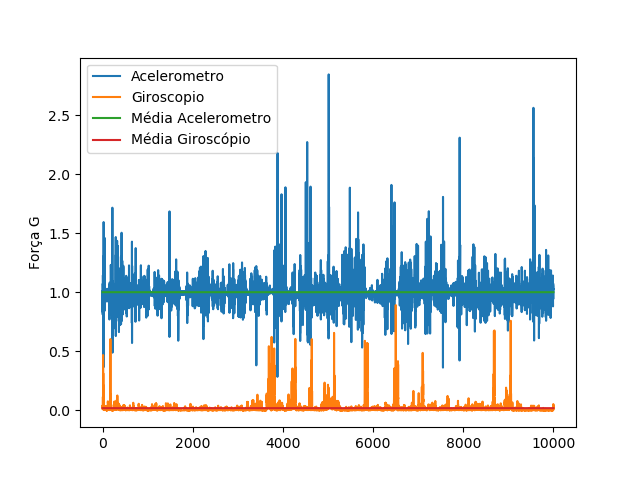
\includegraphics[width=150mm]{images/Cap5/medias_.png}
\end{center}
 \scriptsize Fonte: Os autores
  
\end{figure}



Já para a o protótipo foram adotados os valores do estudo anterior como base, além de teste de quedas para verificar o comportamento dos sensores. Os testes foram realizados em etapas, o celular caiu de alturas específicas dez vezes cada, gerando valores médios dos sensores. Com os dados encontrados nos testes foi  adotada a verificação de acidentes a partir da aceleração resultante para os três eixos do acelerômetro e giroscópio. Foi escolhido utilizar a resultante de todos os eixos pois o celular poderá ficar em qualquer posição junto ao usuário. Então, com isto,  foi definido um \textit{threshold} mínimo para o reconhecimento de acidentes. A Tabela 4 demonstra os  resultados médios adquiridos durante os teste.

\begin{table}[H]
    \centering
    \caption{Valores encontrados para o acelerometro}

\begin{tabular*}{\textwidth}{l@{\extracolsep{\fill}}llllr}
\toprule
{} & Altura(m) & Velocidade Estimada (m/s) & Velocidade Estimada(Km/h) &  Velocidade (Km/h) \\
\midrule
0 &       0,5 &               3,132091953 &               11,27553103 &                                                   15,82346656 \\
1 &         1 &               4,429446918 &               15,94600891 &                                                    18,10074661 \\
2 &       1,5 &               5,424942396 &               19,52979263 &                                                     21,36943805 \\
3 &         2 &               6,264183905 &               22,55106206 &                                                    23,63484279 \\
\bottomrule
\end{tabular*}
\end{table}


Para o acelerômetro foi encontrado um \textit{threshold} de 22 km/h para a detecção de um acidente, com esta velocidade é exercida uma força gravitacional de 5,5G  podendo gerar um acidente leve.

Já para o giroscópio foi considerada a variação da angulação pois é necessário que a variação que haja um \textit{threshold} mínimo para a detecção da queda pois o usuário o irá carregar o celular mesmo estando fora do seu veículo, o próprio ato de caminhar poderia gerar um falso positivo. Com o intuito de remover a detecção de falso positivos foram realizados os seguintes testes da Tabela 5.

Os testes foram utilizados para  chegar um valor específico de \textit{threshold}, sendo assim,  o valor encontrado foi  2.20 km/h.  Esta velocidade mínima do giroscópio é utilizada para remover os falsos positivos sendo acionado somente em batidas leves ou superiores  sendo necessário que ambos os sensores estejam dentro no valor mínimo pré definido em um período de 30 amostras coletadas pelo celular.

\begin{table}[H]
\caption{Tabela de Valores encotrados para o Giroscopio}
\begin{adjustbox}{width=\columnwidth,center}

\begin{tabular}{llrll}
\toprule
{} &  Tipo &  Angulo em  (1 sec) & Velocidade Calculada(m/s) & Velocidade Calculada(Km/h) \\
\midrule
0 &  superfície macia &                   0 &             0,03213005852 &               0,1156682107 \\
1 &  superfície macia &                  90 &              0,7117882769 &                2,562437797 \\
2 &  superfície macia &                 180 &              0,9818256226 &                3,534572241 \\
3 &  superfície macia &                 360 &               1,249420492 &                4,497913771 \\
\bottomrule
\end{tabular}

\end{adjustbox}
\end{table}





\subsection{\textbf{Tempo de Resposta Firebase}}

Para o tempo  de resposta do servidor foram realizados 6 testes com internet móvel e rede \textit{Wifi}, com  e sem  sistema embarcado gerando um acidente. Com este  teste foi possível medir a velocidade de resposta entre eles e verificar qual dos sistemas responde mais rápido.O teste consistiu em utilizar dois celulares e um embarcado, um sendo responsável por receber a notificação e outro por enviar.

O tempo de resposta foi medido a  partir do momento que o celular realiza o envio da  notificação para o servidor até o recebimento da mensagem no outro celular, este intervalo de tempo  para o recebimento da notificação contempla toda a execução do sistema, partindo da primeira requisição sendo coletada  pelo servidor para as realizações de consultas no banco transacional passando para a seleção dos usuários próximos e finalizando na criação do tópico do FCM e realizando o envio para os servidores da \textit{Google}.

Com os valores adquiridos pelos teste foi concluído  que o tempo de resposta utilizando o sistema embarcado é menor, pois assim que o embarcado se comunica com o aplicativo não existe muitos filtros para a autenticação do acidente a não ser por uma validação de sequências de caracteres que definem acidente.Enquanto para o  acionamento do celular está dependente  da variação dos dois sensores sensores e do tempo de aquisição de cada leitura além de que ambos os sensores devem ser acionados em um curto período de tempo para que seja detectado o acidente. A Tabela 6 compara os tempos encontrados.



\begin{table}[H]
    
    \caption{Tabela valores médios do giroscopio e acelerometro}
    \begin{tabular*}{\textwidth}{l@{\extracolsep{\fill}}lllllll}
\toprule
                Tipo &       Conexão & Tempo  1 (s) & Tempo  2 (s) & Tempo  3 (s) \\
\midrule
           Android &  Dados móveis &                    3,57 &                    3,49 &                    3,57  \\
            Android &         WI-FI &                    2,79 &                    2,65 &                     2,7  \\
  Android + Embarcado &  Dados móveis &                    3,28 &                    3,16 &                    3,25  \\
  Android + Embarcado &         WI-FI &                    2,72 &                    2,68 &                    2,78  \\
\bottomrule
\end{tabular*}
\end{table}


\section{SISTEMA EMBARCADO}
O sistema embarcado foi testado quanto à detecção de acidentes em eventos de queda e rotação, bem como em sua comunicação com o dispositivo \textit{Android}. Também foi observado seu consumo de energia como forma de quantizar o tempo de operação nos casos em que o dispositivo não esteja sendo alimentado pelo veículo.

\subsection{\textbf{Quedas}}
O teste de quedas foi realizado a fim de medir a força dos impactos de forma a obter as faixas sensíveis a cada velocidade de impacto. Para os testes foram realizadas três quedas consecutivas de 0.5m, 1m, 1.5m e 2m para cada faixa de sensibilidade pretendida. O teste foi realizado em dois tipos de superfícies sendo a macia (amortecido por colchonete de 3 cm) e rígida (queda sobre o piso). 

Utilizando a equação de Torricelli adaptada para quedas, é possível calcular a velocidade de impacto com base na altura. Ao total foram realizadas 72 quedas. A média obtida entre os valores é demonstrado nas tabelas 7 e 8.

\begin{table}[H]
    \centering
    \caption{Tabela valores médios do giroscopio e acelerometro em superfície macia}
    \begin{tabular*}{\textwidth}{l@{\extracolsep{\fill}}lllllll}
\toprule
{} &                 Altura  &       Velocidade Estimada (km/h) & Queda 1(g) & Queda 2(g) & Queda 3(g) \\
\midrule
0 &              0,5     &   11,28      &        3,522 &                    3,627 &                    3,684  \\
1 &              1 &         15,95 &                    3,947 &                    4,176 &                     3,967  \\
2 &  1,5 &  19,53 &                    4,425 &                    4,39 &                    4,573 \\
3 &  2 &         22,55 &                    4,719 &                    4,759 &                    4,721  \\
\bottomrule
\end{tabular*}


\end{table}


\begin{table}[H]
    \centering
    \caption{Tabela valores médios do giroscopio e acelerometro em superfície rígida}
    \begin{tabular*}{\textwidth}{l@{\extracolsep{\fill}}lllllll}
\toprule
{} &                 Altura  &       Velocidade Estimada (km/h) & Queda 1(g) & Queda 2(g) & Queda 3(g) \\
\midrule
0 &              0,5     &   11,28      &        3,549 &                    3,654 &                    3,632  \\
1 &              1 &         15,95 &                    4,004 &                    4,096 &                     4,044  \\
2 &  1,5 &  19,53 &                    4,551 &                    4,501 &                    4,534 \\
3 &  2 &         22,55 &                    4,911 &                    4,967 &                    4,919  \\
\bottomrule
\end{tabular*}

\end{table}

Os valores para o teste de queda mensurados para ambas superfícies são próximos, porém é possível perceber um aumento da força registrada na superfície rígida em relação a macia conforme é aumentada a altura. Essa maior proximidade dos valores registrados em menores alturas é devido a baixa velocidade a qual o sistema embarcado está sujeito no momento do impacto.


\subsection{\textbf{Rotação}}
O teste de rotação compreende a rotação do dispositivo embarcado de forma a detectar os acidentes por tombamento da motocicleta. Nele foram comparados os ângulos obtidos pelo sistema embarcado com um transferidor, de forma a identificar possíveis variações em suas leituras. Para cada ângulo real o valor foi amostrado três vezes. O resultado dessa análise pode ser visto na tabela 9.


\begin{table}[H]
    \centering
    \caption{Teste de rotação do sistema embarcado}
    \begin{tabular*}{\textwidth}{l@{\extracolsep{\fill}}lllllll}
\toprule
{} &                 Eixo  &       Ângulo esperado (º) & valor 1(º) & valor 2(º) & valor 3(º) \\
\midrule
0 &              X     &   50      &        54 &                    53,7 &                    54,2  \\
1 &              Y &         50 &                    56 &                    55,3 &                     55,6  \\

2 &              X &         60 &                    63,5 &                    63,8 &                     64  \\

3 &              Y &         60 &                    64,8 &                    64,2 &                     64,7  \\

4 &              X &         70 &                    74,3 &                    74,1 &                     73,9  \\

5 &              Y &         70 &                    75,5 &                    75,2 &                     75,7  \\




\bottomrule
\end{tabular*}

\end{table}


A diferença entre o esperado e o mensurado obtido na rotação se deve à posição em que o módulo MPU está posicionado, pois ele se encontra em um pequeno desnível em relação ao ângulo esperado. Esse desnível se deve a natureza de construção do protótipo, sendo seu posicionamento na placa o maior agravante, mas também se deve ao posicionamento e pressão da espuma do preenchimento que pode deslocar-se ligeiramente com os movimentos do veículo.



\subsection{\textbf{Conectividade}}
Foram realizados testes relacionados à conectividade entre o sistema embarcado e o aplicativo \textit{Android}. O teste consistiu no afastamento dos dispositivos com posterior aproximação em 15 tentativas distintas, observando-se assim a reconectividade entre os aparelhos. Nesse teste foram observados os eventos de reconexão bem sucedida, reconexão manual (foi realizado logout e login no aplicativo) e problema crítico (foi necessário realizar um novo pareamento no dispositivo). Os resultados seguem na tabela 10.

\begin{table}[H]
    \centering
    \caption{Teste de conexão entre o sistema embarcado e aplicativo Android}
    \begin{tabular*}{\textwidth}{l@{\extracolsep{\fill}}lllllll}
\toprule
{} &                 Evento  &       Quantidade  & Taxa de reconexão \\
\midrule
0 &              Desconexões     &   15      &       -   \\
1 &              Reconexão automática &         11 &                    73,33\% \\

2 &              Reconexão manual &         3 &                    26,66\%  \\

3 &              Problema crítico &         1 &                    6,66\%   \\

\bottomrule
\end{tabular*}
\end{table}

O problema crítico foi investigado buscando encontrar sua causa. Após testes foi diagnosticado que o problema ocorreu por alguma falha de pareamento onde o embarcado demonstrava que sua conexão estava ativa e funcional, porém o \textit{smartphone} não conseguiu restabeler a conexão. 


\subsection{\textbf{Simulação de acidentes}}

Ao analisar os resultados obtidos nos testes de rotação e queda foi estipulado que a sensibilidade ideal é de 4,3g para a detecção de impactos, o equivalente à detecção de acidentes com velocidade aproximada de 20km/h, e 65º para a rotação. Com estes valores parametrizados foram realizadas mais 20 quedas em cada superfície comentada anteriormente nas alturas de 1m e 1.5m de forma a validar sua detecção.

Das 20 quedas realizadas para cada superfície, foram separadas 10 para cada altura alteriormente comentada. Desse modo as 10 quedas para cada altura foram realizadas sequencialmente, sem interrupções ou reinício de qualquer parte do sistema, com o acompanhamento da detecção de acidentes em tempo real. Os resultados são apresentados na tabela 11.



\begin{table}[H]
\caption{Simulação de acidente com acelerômetro}
\begin{adjustbox}{width=\columnwidth,center}
\begin{tabular}{lllllll}
\toprule
{} &        Superfície     &    Altura (metros)  &       Quantidade & Acerto & falso positivo & falso negativo \\
\midrule
0 &              Macia     &    1         &    10  &  10   &  0 &  0  \\
1 &              Macia     &    1.5       &    10  &  9   &  0 &  1  \\
2 &              Rígida    &    1         &    10  &  8   &  2 &  0  \\
3 &              Rígida    &    1.5       &    10  &  10  &  0 &  0  \\

\bottomrule
\end{tabular}

\end{adjustbox}
\end{table}


Os valores de falso positivo e falso negativo mensurados nos testes foram muito próximos do limiar estipulado. A obtenção desses resultados pode ser atribuída a região de impacto da caixa do sistema embarcado com a superfície, podendo atingir pontos mais macios ou mais rígidos, o que afeta o valor mensurado.

\section{CONSUMO}

\subsection{\textbf{Aplicativo}}

Para o consumo de bateria do \textit{smartphone} foram adotas duas formas de testes. A primeira verifica o consumo da bateria sem a utilização do \textit{Bluetooth} em um período de 8 horas e outro teste conectado com o \textit{Bluetooth} no sistema embarcado no mesmo período de tempo. Para os testes foi considerado o consumo do aplicativo e não o consumo dos módulos habilitados no \textit{Android}.

Para o primeiro teste, considerando que ambos os sensores estavam em operação juntamente com o GPS e rede \textit{WiFi}, foi encontrado um valor de 15 mAh.
Como o teste foi realizado com um \textit{Zenfone} 4 ZE554XL que possui 3300 mAh de autonomia o valor encontrado representa  0,45\% da bateria no período de uma  hora.

Já no segundo teste utilizando novamente GPS,\textit{Wifi} e os sensores com a adição do \textit{Bluetooth} se comunicando com a aplicação, foi encontrado o valor médio de  27 mAh no aplicativo gerando um consumo de 0,81\% do consumo da bateria. A Figura 36 demostra de forma visual o consumo do aparelho para os dois casos.


 \begin{figure}[H]

\begin{center}
     \caption{Consumo de bateria do aplicativo}
  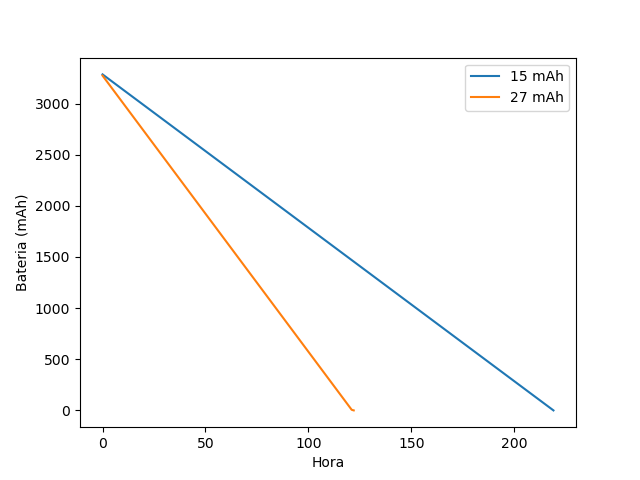
\includegraphics[width=150mm]{images/Cap5/consumo_grafico.png}
\end{center}
 \scriptsize Fonte: Os autores
  
\end{figure}


Analisando os dois casos e considerando uma rotina de  trabalho de um entregador de oito horas sem o \textit{Bluetooth} conectado teria um consumo teórico de 3,6\% e com o \textit{Bluetooth} conectado de  6,48\% sendo assim  um consumo relativamente, baixo sem considerar que muitos motoboys utilizam de power banks para recarregar os celulares enquanto se locomovem pela cidade.









\subsection{\textbf{Sistema embarcado}}

A fim de validar o consumo do sistema embarcado, foi realizada uma pesquisa com o consumo teórico do mesmo, bem como o total real mensurado. Para o módulo MPU-6050 o consumo teórico é de 3.9 mA operando com 6 eixos digitais mais DMP, enquanto para a ESP-32 o consumo teórico de seu processador operando em 240 MHz é de 73 mA, porém com a adição do Bluetooth seu consumo se eleva para 141 mA. O total teórico desconsiderando as perdas do regulador de tensão é de aproximadamente 145 mA, enquanto o valor real mensurado é de 154 mA. A mensuração do valor real foi obtida utilizando um multímetro em série entre o sistema embarcado e uma bateria de moto, levando em consideração o regulador de tensão presente.

Estes valores pesquisados e mensurados para o sistema embarcado foram obtidos apenas por fins de curiosidade, uma vez que o posicionamento do sistema embarcado é no veículo e tem sua alimentação compartilhada com o mesmo.





\section{Conclusão}

Este trabalho apresenta um sistema de monitoramento de acidentes de moto via aplicativo mobile com a extensão de um sistema embarcado. O sistema aposta na política da "boa vizinhança" entre os usuários para seu funcionamento e é responsável por identificar e notificar os usuários de acidentes ocorridos dentro de um raio delimitado. Também é possível adquirir dados relevantes sobre os acidentes como sua data, hora, localização e situação climática.

Com o objetivo de reduzir o tempo de resposta ao prestar os primeiros socorros, o sistema ainda possibilita a visualização dos dados anônimos por parte do público e órgãos competentes permitindo não só uma resposta mais rápida e acertiva quanto aos acidentes motociclisticos como permite a implantação de políticas preventivas em regiões mais perigosas.

Durante a fase de testes foram realizadas avaliações que envolvem todo o ciclo de vida do sistema, compreendendo a criação de um novo usuário e a simulação de acidentes com um ou mais dispositivos dentro do raio determinado. A simulação consistiu em quedas controladas do \textit{smartphone} e do sistema embarcado em momentos distindos, ocasionando a correta ação de notificação de todos os usuário ativos dentro da área delimitada pelo raio traçado a partir do acidentado. No momento do acidente simulado também foi observada a atualização em tempo real dos gráficos e relatórios presentes na plataforma Web.

Ao testar os componentes necessários para o sistema em ambiente controlado, foi possível comprovar a eficácia do sistema em detectar acidentes e notificar todos os usuário próximos em um raio pré-determinado, bem como analisar a rapidez de todos os recursos que necessitam de internet em diferentes cenários, possibilitando assim verificar que os objetivos propostos ao longo deste trabalho foram alcançados.

A plataforma Web contendo relatórios possibilita uma simples visualização dos dados sobre acidentes, permitindo que outros serviços possam utilizá-los. Nesse sentido o sistema prova-se uma alternativa eficiente não só em reduzir o tempo de resposta para os primeiros socorros em casos se acidente, mas também arquiva e disponibiliza dados que podem ser utilizados em políticas de prevenção e assistência.




\clearpage

\section{Trabalhos Futuros}

Como possíveis trabalhos futuros, pode-se apontar:

\begin{enumerate}
    \item Enriquecer os dados adquiridos com as informações do sensores para criar uma base para análise preditiva de acidentes em regiões específicas, horários ou tipo de clima.
    
    \item Integrar o sistema com os órgãos  públicos gerando análises de comportamento de trânsito, regiões perigosas por hora e clima sendo possível verificar a velocidade do tráfego por região aumentando a fiscalização ou ajustando os limites das vias.
    
    \item Para empresas privadas é possível realizar todo o rastreio da frota de veículos de entrega, sendo capaz de verificar o desempenho de cada usuário em situações diferenciadas como em dia chuvosos, nublados e além de poder fazer todo um rastreio da rota realizada por usuário sendo capaz de realizar otimização de rotas de entregas e distribuição das entregas para os usuários com mais aptidão em tipos de climas ou horários especificos.
    
\end{enumerate}









